\documentclass[../Cours.tex]{subfiles}

\begin{document}
\clearpage
\thispagestyle{empty}

\color{black}
\addcontentsline{toc}{chapter}{\textcolor{rouge}{Épreuve commune (entraînement)}}%
\addcontentsline{toc}{section}{\textcolor{vert}{Sujet}}%

\begin{center}
    \Huge{Épreuve commune de $4^{\mbox{ème}}$ (entraînement)}
\end{center}

\begin{questions}

\exercice
Chaque question ne contient \textbf{qu'une seule bonne réponse}, et ne nécessite \textbf{aucune justification}.

\begin{center}
\begin{tabularx}{\linewidth}{|l|C|C|C|C|} \hline
    Question & A & B & C & D \\\hline \hline 
    \makecell[l]{Dans laquelle de ces figures les \\deux droites sont parallèles ?}
    & 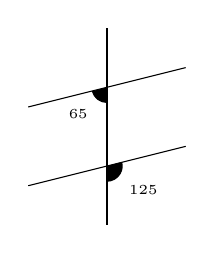
\begin{tikzpicture}
        \draw (0,0) -- (2,0.5);
        \draw (0,-1) -- (2,-0.5);
        \draw (1,1) -- (1,-1.5);
        \fill[black] (1,-0.75) -- ++(0,-0.2) arc(-90:15:0.2) node[midway,below right]{\tiny{\ang{125}}} -- cycle;
        \fill[black] (1,0.25) -- ++(0,-0.2) arc(-90:-165:0.2) node[midway,below left]{\tiny{\ang{65}}} -- cycle;
    \end{tikzpicture}
    & 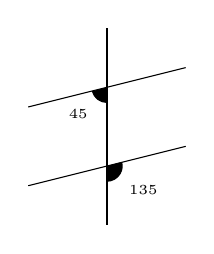
\begin{tikzpicture}
        \draw (0,0) -- (2,0.5);
        \draw (0,-1) -- (2,-0.5);
        \draw (1,1) -- (1,-1.5);
        \fill[black] (1,-0.75) -- ++(0,-0.2) arc(-90:15:0.2) node[midway,below right]{\tiny{\ang{135}}} -- cycle;
        \fill[black] (1,0.25) -- ++(0,-0.2) arc(-90:-165:0.2) node[midway,below left]{\tiny{\ang{45}}} -- cycle;
    \end{tikzpicture}
    & 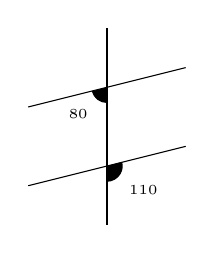
\begin{tikzpicture}
        \draw (0,0) -- (2,0.5);
        \draw (0,-1) -- (2,-0.5);
        \draw (1,1) -- (1,-1.5);
        \fill[black] (1,-0.75) -- ++(0,-0.2) arc(-90:15:0.2) node[midway,below right]{\tiny{\ang{110}}} -- cycle;
        \fill[black] (1,0.25) -- ++(0,-0.2) arc(-90:-165:0.2) node[midway,below left]{\tiny{\ang{80}}} -- cycle;
    \end{tikzpicture}
    & 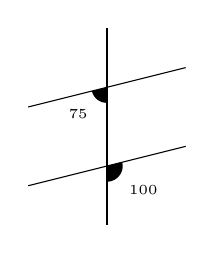
\begin{tikzpicture}
        \draw (0,0) -- (2,0.5);
        \draw (0,-1) -- (2,-0.5);
        \draw (1,1) -- (1,-1.5);
        \fill[black] (1,-0.75) -- ++(0,-0.2) arc(-90:15:0.2) node[midway,below right]{\tiny{\ang{100}}} -- cycle;
        \fill[black] (1,0.25) -- ++(0,-0.2) arc(-90:-165:0.2) node[midway,below left]{\tiny{\ang{75}}} -- cycle;
    \end{tikzpicture} \\\hline
    \makecell[l]{Lequel de ces nombres \\n'est pas divisible par 9 ?} & 784 &  4995 & 1566 & 88884 \\\hline
    \makecell[l]{Deux amis ont joué au loto et leur mise \\s’est faite selon le ratio 3:5. \\Ils gagnent 64 euros. Quelle est la somme\\d’argent qui revient à chacun d’eux ?} & \qty{3}{\EURO} et \qty{5}{\EURO} & \qty{24}{\EURO} et \qty{40}{\EURO} & \qty{40}{\EURO} et \qty{24}{\EURO} & \qty{5}{\EURO} et \qty{3}{\EURO} \\\hline
    \makecell[l]{Soit la série de nombres \{15 ; 10 ; 13 ; 9 ; 10\}\\ La moyenne de la série est ...} & \num{11.2} & \num{11.4} & \num{11.6} & \num{11.8} \\\hline
\end{tabularx}
\end{center}

\exercice
Sur la figure ci-dessous, $C$ est un point du demi-cercle de diamètre $[PR]$ tel que $CR=\qty{1500}{\milli\metre}$. Le triangle $RCP$ est rectangle en $C$.

\begin{centre}
    \begin{tikzpicture}[scale=1.5]
        \draw (-1.5,0) arc(180:0:1.5);
        \draw (-1.5,0) node[left]{$R$} -- ({1.5*cos(120)},{1.5*sin(120)}) node[above left]{$C$} -- (1.5,0) node[right]{$P$} -- cycle;
        \draw[Latex-Latex] (-1.5,-0.15) -- +(3,0) node[midway,below]{\qty{3000}{\milli\metre}};
        \fill[black,rotate around={-120:({1.5*cos(120)},{1.5*sin(120)})}] ({1.5*cos(120)},{1.5*sin(120)}) rectangle +(0.1,0.1);
    \end{tikzpicture}
\end{centre}

\question Calculer la distance $PC$.
\question En déduire l'aire du triangle $RCP$.

\exercice
Voici un programme de calcul.

\begin{center}
    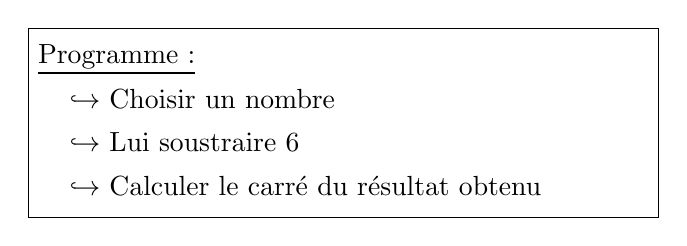
\begin{tikzpicture}
        \draw (0,0.5) rectangle +(8,2.4);
        \node[anchor=west] at (0,2.5) {\underline{Programme :}};
        \node[anchor=west] at (0.4,2) {$\hookrightarrow$ Choisir un nombre};
        \node[anchor=west] at (0.4,1.45) {$\hookrightarrow$ Lui soustraire 6};
        \node[anchor=west] at (0.4,0.9) {$\hookrightarrow$ Calculer le carré du résultat obtenu};
    \end{tikzpicture}
\end{center}

\question Si on choisit le nombre 4 au départ, montrer que le résultat obtenu est 4.
\question On choisit 15 comme nombre de départ, quel est le résultat obtenu ?
\question Si, en réalisant le programme, on obtient 144, quel nombre a-t-on choisi au départ ?
\question 
    \subquestion Réaliser le programme en choisissant $x$, quelle expression littérale obtient-on ?
    \subquestion Montrer que cette expression littérale est aussi égale à $x^2-12x+36$.

\exercice
Mathilde est une élève de quatrième qui mesure \qty{1.55}{\metre} et qui souhaite déterminer la hauteur d'un cocotier. Elle a vu en cours de mathématiques que l'on pouvait utiliser son ombre pour calculer la hauteur d'un objet trop grand pour les outils classiques.\\ 

Dans la figure ci-dessous, les points $B$, $D$ et $C$ sont alignés, et les points $B$, $E$, $A$ sont alignés.

\begin{center}
    \begin{tikzpicture}[scale=1.4]
        \coordinate (A) at (0,0);
        \coordinate (B) at (7,0);
        \coordinate (C) at (0,3);
        \coordinate (D) at ($(B)!0.5!(C)$);
        \coordinate (E) at ($(B)!(D)!(A)$);
        \draw (A) -- (B) -- (C) -- cycle;
        \draw (D) -- (E);
        \node[left] at (A) {$A$};
        \node[right] at (B) {$B$};
        \node[left] at (C) {$C$};
        \node[above] at (D) {$D$};
        \node[below] at (E) {$E$};
        \draw[Latex-Latex] ($(A)+(0,-0.2)$) -- ($(E)+(-0.2,-0.2)$) node[midway,below]{\qty{7}{\metre}};
        \draw[Latex-Latex] ($(E)+(0.2,-0.2)$) -- ($(B)+(-0.2,-0.2)$) node[midway,below]{\qty{3}{\metre}};
        \node[above,rotate=90] at ($(A)!0.5!(C)$) {cocotier};
        \draw[Latex-Latex] (C) ++(-0.5,0) -- ++(0,-3) node[midway,left]{?};
        \node[above,rotate=90] at ($(D)!0.5!(E)$) {Mathilde};
    \end{tikzpicture}
\end{center}

\question Calculer la hauteur du cocotier.

\exercice
A l'entrée d'un parc d'attractions figurent les informations suivantes :

\begin{center}
    \begin{tabularx}{0.9\linewidth}{|l|X|}\hline
    \textbf{Tarifs} & \textbf{Horaires} \\\hline
    Entrée adulte : \qty{12}{\EURO} & Ouvert de \qty{9}{\hour} à \qty{18}{\hour} \\\hline
    Entrée enfant : \qty{7}{\EURO} & Dernières entrées à \qty{17}{\hour} \\\hline
    Forfait famille (sur présentation du livret de famille) : \qty{35}{\EURO} & Fermé le lundi \\\hline
    \end{tabularx}
\end{center}

\question
    \subquestion Est-il intéressant pour un couple et leur enfant de 8 ans de prendre le forfait famille ?
    \subquestion À partir de quel nombre d'enfants un couple a-t-il intérêt à choisir le forfait famille ?
\question Au cours d'une journée, 89 forfaits famille ont été vendus pour 510 personnes.
    \subquestion Déterminer la recette correspondante.
    \subquestion Quel est le prix moyen par personne ?

\exercice

La vitesse est mise en cause dans près d’un accident mortel sur deux.\\
Un cyclomoteur est conçu pour ne pas dépasser une vitesse de \qty{45}{\kilo\metre\per\hour}. Si le moteur est gonflé au-delà de la puissance légale, les freins et les pneus ne sont plus adaptés et le risque d’accident augmente alors considérablement.\\

Léa et Gérard ont chacun un scooter. Ils doivent rejoindre leurs amis à la piscine qui est à \qty{8}{\kilo\metre} de chez eux.

\question Léa roule en moyenne à \qty{40}{\kilo\metre\per\hour}. Combien de temps mettra-t-elle pour aller à la piscine ? Donner le résultat en minutes.
\question Gérard est plus pressé, il roule en moyenne à \qty{48}{\kilo\metre\per\hour}. Calculer le temps qu'il mettra pour aller à la piscine. Donner le résultat en minutes.
\question Combien de temps Gérard a-t-il gagné par rapport à Léa ? 
\question Pourquoi Gérard a pris des risques par rapport à Léa ? Cela valait-il le coup ?

\end{questions}
\end{document}